\documentclass[letterpaper]{article}
\usepackage[letterpaper]{geometry}
\usepackage{hyperref}
\usepackage{amsmath}
\usepackage{graphicx}

%opening
\title{CS 7641 --- Assignment 2: Randomized Search}
\author{Niranjan Thakurdesai}

\begin{document}
	\maketitle
	
	\section{Local random search for finding neural network weights}
	Three local random search algorithms, viz. randomized hill climbing (RHC), simulated annealing (SA) and a genetic algorithm (GA) were used to train the neural network used in assignment 1.
	
	\subsection{The network}
	The network has two hidden layers with 5 and 2 nodes respectively and ReLU activations. The cross-entropy loss function with regularization was used for training, i.e. the random search algorithms tried to minimize this loss.
	
	\subsection{Data}
	The Breast Cancer Wisconsin (Diagnostic) Data Set provided by UCI Machine Learning which was used in assignment 1 has been used here as well. Given features computed from a digitized image of a fine needle aspirate (FNA) of a breast mass, the task is to predict the diagnosis of the tissue (benign or malignant). The class distribution is as follows: 62.74\% benign (negative), 37.26\% malignant (positive).
	
	\subsection{The benchmark: Gradient Descent}
	In assignment 1, the above neural network was trained with gradient descent. The best accuracy obtained on the test set was 98.25\%. It would be interesting to see how the random search algorithms perform w.r.t. this benchmark.
	
	\subsection{Implementation}
	RHC and SA were implemented in Python from scratch. For GA, the ABAGAIL\footnote{\url{https://github.com/pushkar/ABAGAIL}} library was used with Jython.
	
	\subsection{Randomized Hill Climbing}
	The implementation closely follows the pseudocode given in the slides. The Glorot initialization\cite{glorotUnderstandingDifficultyTraining} of the network weights was used as the initial guess. The weights are randomly perturbed simultaneously by adding a random number uniformly distributed between $[-\Delta, \Delta]$. Here, $\Delta$ is the maximum step size. If the perturbed weights reduce the loss, the update is accepted. Otherwise, the weights are perturbed again. This is repeated until the reduction in loss is below a certain threshold or the maximum number of iterations is reached. Random restarts are used and the best set of weights across the runs is chosen.
	
	\subsubsection{Experiments}
	Different step sizes in a log-linear scale in $[10^{-6}, 1]$ were tried out and it was found that a step size of 0.1 provides good convergence. Hence, this step size was used in further experiments. The maximum number of iterations was set to 5000 and the threshold for convergence was set to $10^{-5}$.
	
	\subsubsection{Analysis}
	\begin{figure}
		\centering
		\begin{minipage}{.5\textwidth}
			\centering
			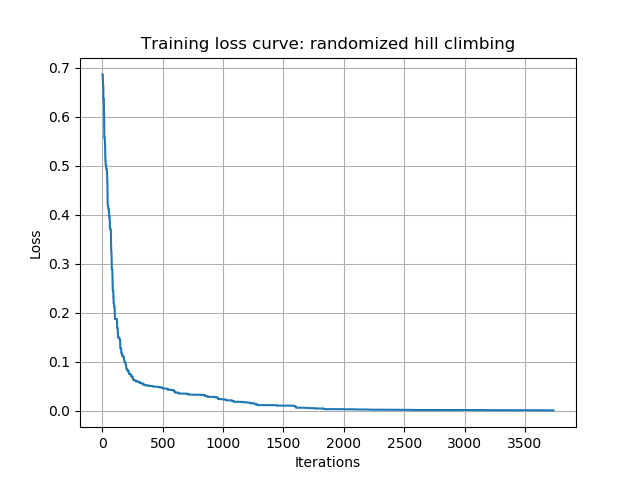
\includegraphics[width=\linewidth]{../plots/nn_loss_rhc}
			\caption{Loss curve for RHC}
			\label{fig:rhc_loss}
		\end{minipage}%
		\begin{minipage}{.5\textwidth}
			\centering
			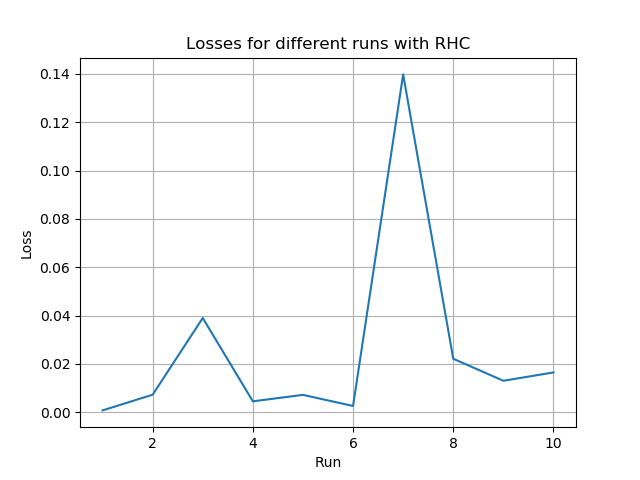
\includegraphics[width=\linewidth]{../plots/nn_runs_rhc}
			\caption{Loss for different runs of RHC}
			\label{fig:rhc_runs}			
		\end{minipage}
	\end{figure}
	The test accuracy obtained with the best set of weights was 97.37\%. The loss curve for a particular RHC run is plotted in figure \ref{fig:rhc_loss}. We can observe that the loss slowly converges towards zero. The tiny flat regions in the curve indicate that a suboptimal neighbor was chosen due to which the loss did not decrease. The losses for different RHC runs are plotted in figure \ref{fig:rhc_runs}. We can see that the losses are not the same for each run due to the stochastic nature of the algorithm. Moreover, RHC can get stuck in local optima which can be observed in some runs where the loss is high. One run of RHC took 2.4 seconds on an average.
	
	\subsection{Simulated Annealing}
	The initial temperature is set to be a high value and is slowly decreased according to a decay rate. The Metropolis criterion\cite{vanlaarhovenSimulatedAnnealing1987} is used for updating weights. The weights are perturbed by adding a random number uniformly distributed between $[-\Delta, \Delta]$. Here, $\Delta$ is the maximum step size. After each iteration, the temperature is decayed by multiplying with a constant factor less than 1.
	
	\subsubsection{Experiments}
	The initial temperature and the decay rate were tuned to $10^{5}$ and $0.95$ after observing convergence. The maximum number of iterations was set to 5000.
	
	\subsubsection{Analysis}
	\begin{figure}
		\centering
		\begin{minipage}{.5\textwidth}
			\centering
			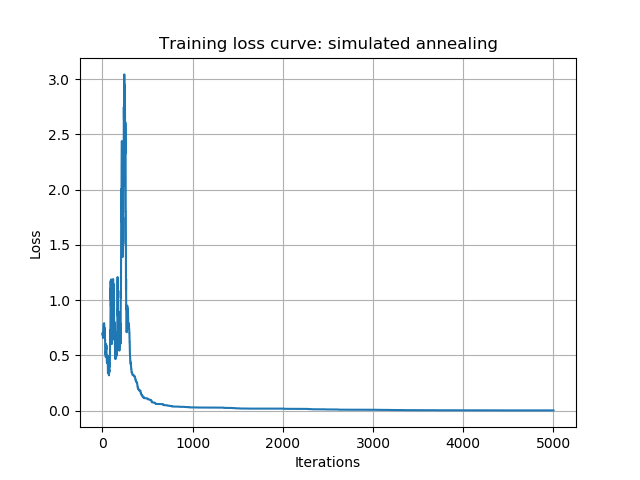
\includegraphics[width=\linewidth]{../plots/nn_loss_sa}
			\caption{Loss curve for SA}
			\label{fig:sa_loss}
		\end{minipage}%
		\begin{minipage}{.5\textwidth}
			\centering
			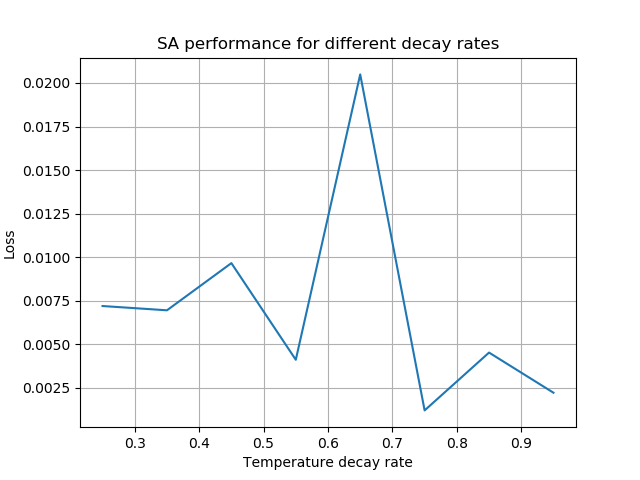
\includegraphics[width=\linewidth]{../plots/nn_sa_decay_rates}
			\caption{Loss for different SA decay rates}
			\label{fig:sa_decay}			
		\end{minipage}
	\end{figure}
	The test accuracy obtained with SA was 96.93\%. The time taken to run was 6.45 seconds. The loss curve is plotted in figure \ref{fig:sa_loss}. SA can accept locally bad moves with a high probability when the temperature is high. We can observe this behavior in the plot where there are a large number of fluctuations initially. As the number of iterations increases, the temperature goes down and it becomes increasingly unlikely to accept locally bad moves. This can be observed in the plot for later iterations where loss smoothly decreases.
	
	The training loss and the test accuracy with different temperature decay rates is plotted in figure \ref{fig:sa_decay}. To retain optimality, the temperature has to be decreased very gradually. Thus, the decay rate cannot be too small. We can observe in the plot that the loss increases as the decay rate decreases. This demonstrates that if the cooling is not done slowly, SA can get stuck in local minima.
	
	\subsection{Genetic Algorithm}
	A population of network weights is initialized by randomly sampling numbers in $[-0.5, 0.5]$ uniformly. In each iteration, a probability distribution is calculated over the population. The probability of each individual is proportional its loss. This distribution is then used for crossovers and mutations. The higher the loss of an individual, the greater its probability of being picked for crossover or mutation. The sampling is done with replacement. In each iteration, a fixed number of crossovers and mutations are carried out to form a new population which is passed on to the next iteration. This procedure runs for a fixed number of iterations.
	
	\subsubsection{Experiments}
	The population size, the number of crossovers and the number of individuals mutated per iterations were chosen to be 200, 100 and 10 respectively. An extensive hyperparameter search was not done as running GA is expensive and good performance was obtained with the above settings. The maximum number of iterations was set to 1000.
	
	\subsubsection{Analysis}
	\begin{figure}
		\centering
		\begin{minipage}{\textwidth}
			\centering
			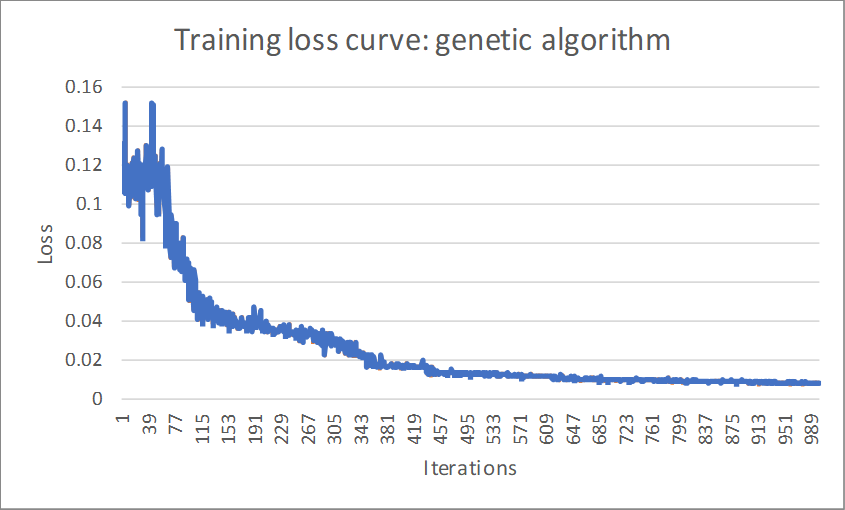
\includegraphics[width=.6\linewidth]{../plots/nn_loss_ga}
			\caption{Loss curve for GA}
			\label{fig:ga_loss}
		\end{minipage}
	\end{figure}
	A test accuracy of 97.81\% was obtained with GA. The time taken to run was 37.57 seconds. The loss curve is plotted in figure \ref{fig:ga_loss}. The loss slowly converges as an increasing number of individuals in the population reach the basin around a local/global optimum. Like SA, GA can also accept locally bad moves, resulting in the fluctuations in losses in the initial iterations.
	
	\subsection{Comparison}
	\label{sec:nn_comp}
	\begin{figure}
		\centering
		\begin{minipage}{.5\textwidth}
			\centering
			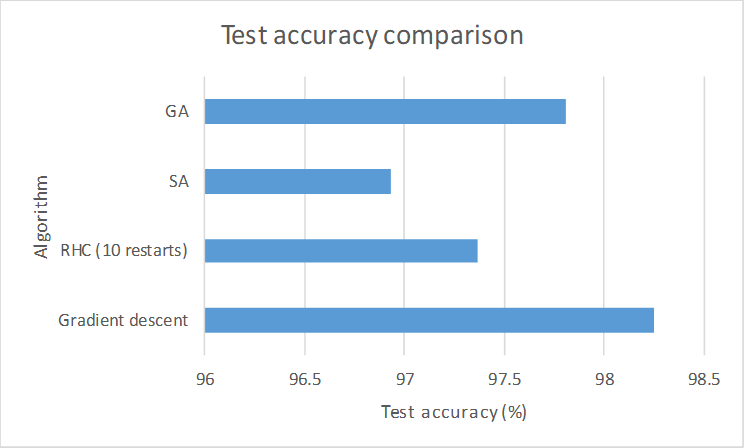
\includegraphics[width=\linewidth]{../plots/nn_acc_comparison}
			\caption{Comparison of accuracy}
			\label{fig:comp_acc}
		\end{minipage}%
		\begin{minipage}{.5\textwidth}
			\centering
			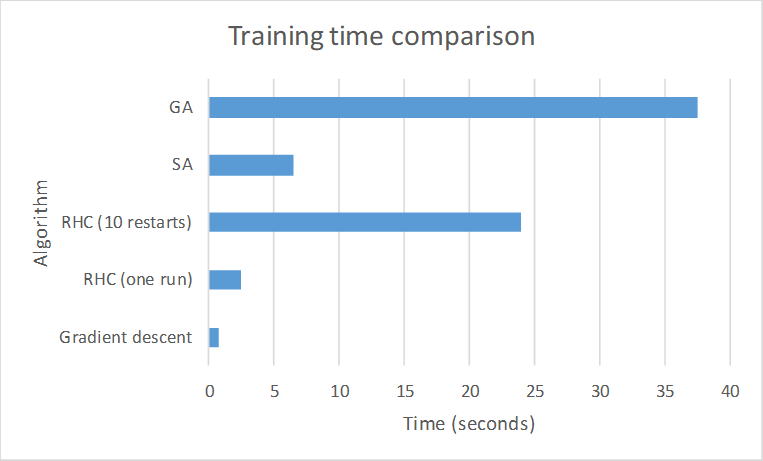
\includegraphics[width=\linewidth]{../plots/nn_time_comparison}
			\caption{Comparison of training time}
			\label{fig:comp_time}			
		\end{minipage}
	\end{figure}
	The performance of the three random search algorithms and gradient descent is compared in figures \ref{fig:comp_acc} and \ref{fig:comp_time}. Among the random search algorithms, GA gives the best test accuracy, possibly because it explores a larger part of the solution space compared to the others. However, it is computationally expensive because each iteration requires population size number of function evaluations compared to only one in case of RHC and SA. SA gives the worst performance, possibly because of getting stuck in a local optimum at a low temperature. SA takes lesser time than GA but more than a single run of RHC because of the Metropolis criterion evaluation in each iteration. RHC performs better than SA but worse than GA possibly because it got stuck in a local optimum which it is prone to. A single run of RHC requires the least amount of time among the random search algorithms. However, if restarts are taken into account, its time exceeds that of SA but is still lesser than GA.
	
	Gradient descent, on the other hand, gives the best test accuracy among all the algorithms while also taking the least amount of time to run. This might be because following the direction of steepest descent from the Glorot initialization quickly led to the global optimum. The random search algorithms do not use a gradient and might have explored suboptimal solution spaces.
	
	However, one should keep in mind that the network used here was relatively small (only 2 hidden layers with 5 and 2 nodes). Increasing the dimensionality of the search space might put random search algorithms to an advantage as they have a greater chance of escaping global minima than gradient descent. However, this is at the expense of more computation.
	
	To improve the performance of the random search algorithms, cross-validation could be used to tune their hyperparameters (e.g. step size for RHC, initial temperature and decay rate for SA, population size, number of crossovers and mutations for GA).
	
	\section{Optimization Problems}
	Two optimization problems are presented in this section. The first problem highlights the advantages of using a genetic algorithm and the second of simulated annealing.
	
	Both problems use bitstrings. Any string with a Hamming distance of 1 is a neighbor. For GA, single point crossovers are used to create offspring. Mutations are carried out by flipping a randomly chosen bit.
	
	\subsection{Four Peaks Problem (GA)}
	\label{sec:4peaks}
	Four Peaks is a toy problem designed by Baluja and Caruana\cite{balujaRemovingGeneticsStandard1995} to be GA-friendly. Given an $N$-dimensional bitstring $\mathbf{x}$, the four peaks evaluation function is given by:
	\begin{align*}
		f(\mathbf{x}, T) &= \max\{tail(0, \mathbf{x}), head(1, \mathbf{x})\} + R(\mathbf{x}, T) \\
		\text{where} \\
		tail(0, \mathbf{x}) &= \text{number of trailing 0's in } \mathbf{x} \\
		head(1, \mathbf{x}) &= \text{number of leading 1's in } \mathbf{x} \\
		R(\mathbf{x}, T) &= 
		\begin{cases}
		N, & \text{if } tail(0, \mathbf{x}) > T \text{ and } head(1, \mathbf{x}) > T \\
		0 & \text{otherwise}
		\end{cases}
	\end{align*}
	
	This function has two global maxima, achieved either when there are $T+1$ trailing 0's preceded by all 1's or when there are $T+1$ leading 1's followed by all 0's. Such a string achieves the maximum value of both the ``reward" $R$ and length of one of head or tail. For example, if $N = 100$ and $T = 10$, the optimal fitness 189 is obtained by strings containing either eighty-nine 1's followed by eleven 0's or eleven 1's followed by eighty-nine 0's. In general, the fitness at the global maximum is given by $N + N - (T + 1) = 2N - T - 1$ Note that strings with lengths of head and tail greater than $T$ but sub-optimal can reach one of the global maxima by repeatedly flipping bits at the end of the head or the beginning of the tail, whichever is largest. For example, if $tail(0, \mathbf{x}) = 40$ and $head(1, \mathbf{x}) = 20$, the global maximum at $tail(0, \mathbf{x}) = 89$ and $head(1, \mathbf{x}) = 11$ can be reached by flipping the 41st bit to 0, then the 42nd bit and so on.
	
	There are also two local maxima with a fitness of $N$ that occur with a string of all 1's or all 0's. RHC and SA will get trapped in these local maxima. For example, if $N = 100$, $tail(0, \mathbf{x}) = 20$ and $head(1, \mathbf{x}) = 5$, RHC and SA will continue to increase the value of the tail until it is 100. The only way a string with both head and tail less than $T$ to reach a global maximum is if it keeps flipping bits at the shorter end even when the fitness is not improving. This is extremely unlikely to happen with SA even if it sometimes accepts parameter updates which don't improve fitness. RHC cannot do this because it updates parameters only if the fitness improves.
	
	GA can overcome this problem through crossover. Crossover on a population of strings, some of which have $head(1, \mathbf{x}) >> tail(0, \mathbf{x})$ and others which have $tail(0, \mathbf{x}) >> head(1, \mathbf{x})$ but none of them with $head(1, \mathbf{x}) > T$ and $tail(0, \mathbf{x}) > T$, is likely to create individuals with $head(1, \mathbf{x}) > T$ and $tail(0, \mathbf{x}) > T$. When this happens, the child string will receive the additional reward of $N$ and will have a higher fitness than its parents.
	
	\subsubsection{Experiments}
	\label{sec:fourpeaks_exp}
	The ABAGAIL library was used with Jython for the implementation of the three algorithms. Each algorithm was run for 200,000 iterations to provide a fair comparison. For SA, the initial temperature was set to $10^{11}$ and the decay rate was 0.95. For GA, the population size was 200, the number of crossovers in each iteration was 100 and the number of individuals mutated was 10. The number of bits in the string ($N$) was varied from 20 to 100 with increments of 10 and $T$ was set to be $N/5$. Each algorithm was randomly restarted 10 times and the best performance over all runs is reported for each value of $N$.
	
	\subsubsection{Analysis}
	\begin{figure}
		\centering
		\begin{minipage}{.5\textwidth}
			\centering
			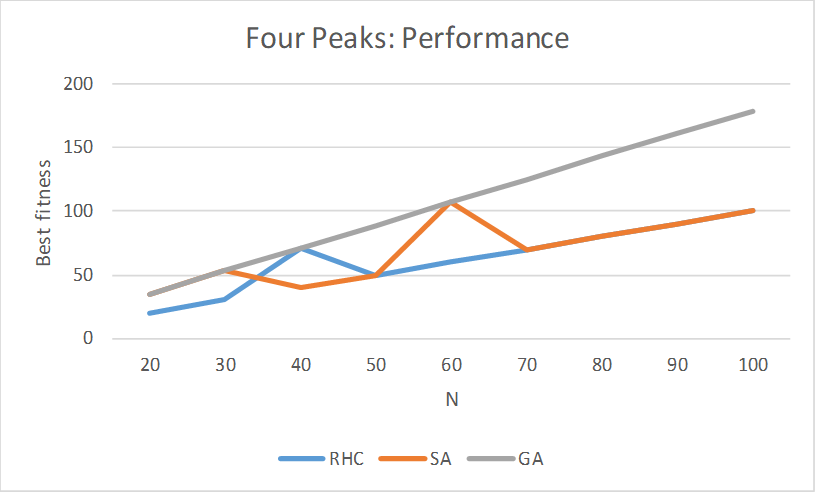
\includegraphics[width=\linewidth]{../plots/fourpeaks_fitness}
			\caption{Performance on Four Peaks}
			\label{fig:fourpeaks_fitness}
		\end{minipage}%
		\begin{minipage}{.5\textwidth}
			\centering
			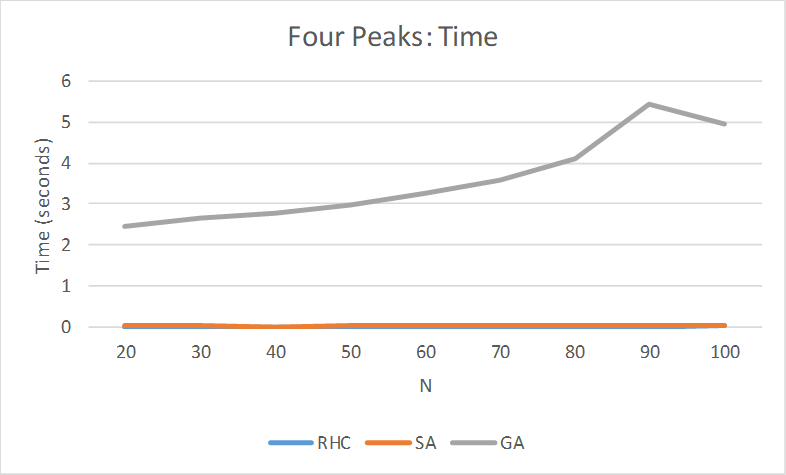
\includegraphics[width=\linewidth]{../plots/fourpeaks_time}
			\caption{Time taken to solve Four Peaks}
			\label{fig:fourpeaks_time}			
		\end{minipage}
	\end{figure}
	The best performance for different bitstring sizes for each algorithm is plotted in figure \ref{fig:fourpeaks_fitness}. As expected, GA outperforms RHC and SA for all values of $N$. As explained in section \ref{sec:4peaks}, GA is able to exploit the structure of the solution space through crossovers and reach the global maxima whereas RHC and SA get stuck in local maxima. For some low values of $N$, RHC and SA are also able to reach the global optimum. This is possibly because the basins of attraction around the global maxima are large enough compared to those around local maxima for RHC and SA to catch them and move to the global maxima. However, as $N$ increases, the basins of attraction around the local maxima become wider and it is extremely likely that RHC and SA get stuck in them.
	
	However, GA achieves better performance at the expense of computation time. As observed in figure \ref{fig:fourpeaks_time}, GA takes a lot more time than RHC and SA due to reasons explained in section \ref{sec:nn_comp}.
	
	\subsection{Continuous Peaks}
	This problem is an extension of Four Peaks highlights the strength of SA. Rather than forcing 1's and 0's to be at the ends of the string, they are allowed to form anywhere in the string. A reward is given when there are greater than $T$ contiguous bits set to 0, and greater than $T$ contiguous bits set to 1. It has many local maxima. Unlike Four Peaks, this problem doesn't have a structure which can be exploited through crossovers and we expect SA to work better than GA.
	
	\subsubsection{Experiments}
	Each algorithm was run for 200,000 iterations to provide a fair comparison. $N$ was varied from 50 to 200 with increments of 25 and $T$ was set to be $N/10$. Other settings are the same as Four Peaks (described in section \ref{sec:fourpeaks_exp}).
	
	\subsubsection{Analysis}
	\begin{figure}
		\centering
		\begin{minipage}{.5\textwidth}
			\centering
			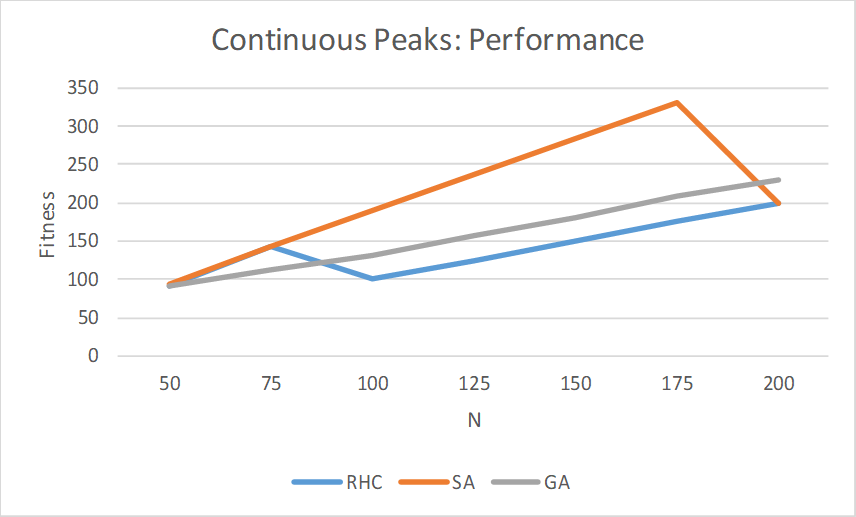
\includegraphics[width=\linewidth]{../plots/continuouspeaks_fitness}
			\caption{Performance on Continuous Peaks}
			\label{fig:contpeaks_fitness}
		\end{minipage}%
		\begin{minipage}{.5\textwidth}
			\centering
			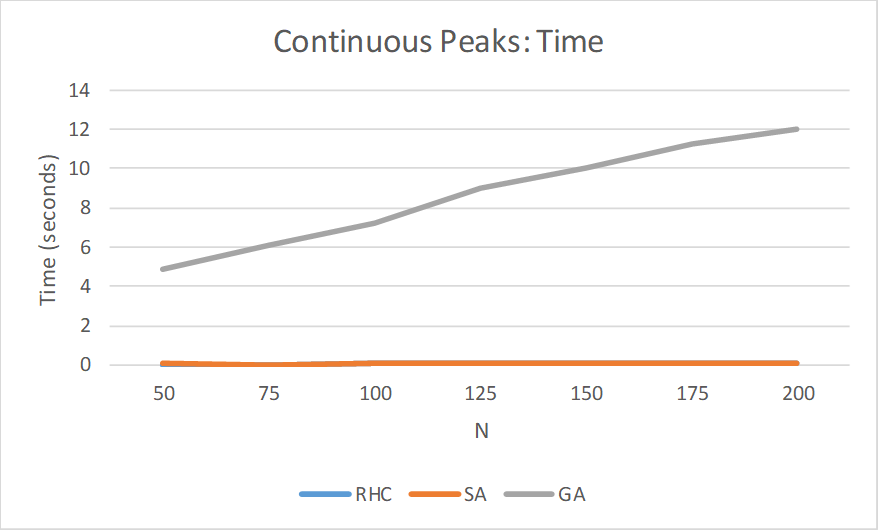
\includegraphics[width=\linewidth]{../plots/continuouspeaks_time}
			\caption{Time taken to solve Continuous Peaks}
			\label{fig:contpeaks_time}			
		\end{minipage}
	\end{figure}
	As observed in figure \ref{fig:contpeaks_fitness}, SA performs the best for all values of $N$ except 200. At such a high value, it is possible that SA did not explore the solution space enough at higher temperatures and converged to the local optimum as the temperature decreased. RHC performs as good as SA initially but its performance falls off later. Like the previous problem, GA has the most computation time followed by SA and RHC.
	
	\subsection{Conclusion}
	As we saw above, there are some problem domains which are more suited to certain randomized optimization algorithms. It would be instructive to see if it is possible to theoretically characterize these domains. The above experiments demonstrate that before choosing a randomized optimizaton algorithm to solve a particular problem, it is useful to have knowledge of the domain and the structure of the solution space to decide which algorithm would have a higher chance of success.
	
	\bibliographystyle{unsrt}
	\bibliography{cs7641-assgn2}
	
\end{document}
